\documentclass{article}
\usepackage{polski}
\usepackage[utf8]{inputenc}
\usepackage{graphicx}
\usepackage{amsmath}
\usepackage{amssymb}
\usepackage{mathtools}
\usepackage{hyperref}
\usepackage{enumerate}
% \usepackage{}
\title{Teoria Regulacji - Ćwiczenia}
\author{Jan Bronicki 249011}
\date{}

\begin{document}

\maketitle


\section*{Zadanie 2}
\begin{enumerate}[a)]
    \item Hurwitz 
    \begin{enumerate}[a)]
        \item $K_{o}\left(o\right)=\frac{1}{\left(s+1\right)\left(s+2\right)\left(s+3\right)}
        , \ K_{k}\left(s\right)=k$
        
        $$K_{OTW}\left(s\right)=\frac{k}{s^{3}+6s^{2}+11s+6}$$
        
        $$ M_{UAR}=L_{OTW}\left(s\right)+M_{OTW}\left(s\right)=
        \left(s+1\right)\left(s+2\right)\left(s+3\right)+k=s^{3}+6s^{2}+11s+6+k $$
        
        $$H_{3}=\left[\begin{matrix}
            6 & 6+k & 0   \\
            1 & 11  & 0   \\
            0 & 6   & 6+k
        \end{matrix}\right]$$
        
        \[\begin{cases}
            \Delta_{1}=6>0
            \\
            \Delta_{2}=60+k>0 \rightarrow k>-60
            \\
            \Delta_{3}=\left(6+k\right)\cdot \Delta_{2}=\left(6+k\right) \left(60+k\right) \rightarrow k>-6 \ lub \ k<-60
        \end{cases}\]
        
        $$k \in \left(-6, 60\right)$$
        
        \item $K_{o}\left(s\right)=\frac{1}{\left(s+1\right)^{2}\left(s+2\right)}, \ K_{R}\left(s\right)=k$
        
        $$ K_{OTW}\left(s\right)=\frac{k}{\left(s+1\right)^{2}\left(s+2\right)}$$
        
        $$M_{UAR}\left(s\right)=L_{OTW}\left(s\right)+M_{OTW}\left(s\right)=s^{3}+4s^{2}+5s+2+k $$
        
        
        $$H_{3}=\left[\begin{matrix}
            4 & 2+k & 0   \\
            1 & 5  & 0   \\
            0 & 4   & 2+k
        \end{matrix}\right]$$
        
        \[\begin{cases}
            \Delta_{1}=4>0
            \\
            \Delta_{2}=18-k>0 \rightarrow k<18
            \\
            \Delta_{3}=\left(2+k\right)\cdot \Delta_{2}=\left(2+k\right) \left(18-k\right) \rightarrow k>-2 \ lub \ k<18
        \end{cases}\]
        
        $$k \in \left(-2, 18\right)$$
    \end{enumerate}
    
    \newpage

    \item Nyquist
    
    \begin{enumerate}[a)]
        \item $K_{OLS}=\frac{k}{\left(s + 1\right) \left(s + 2\right) \left(s + 3\right)}$
        
        \begin{figure}[h!]
            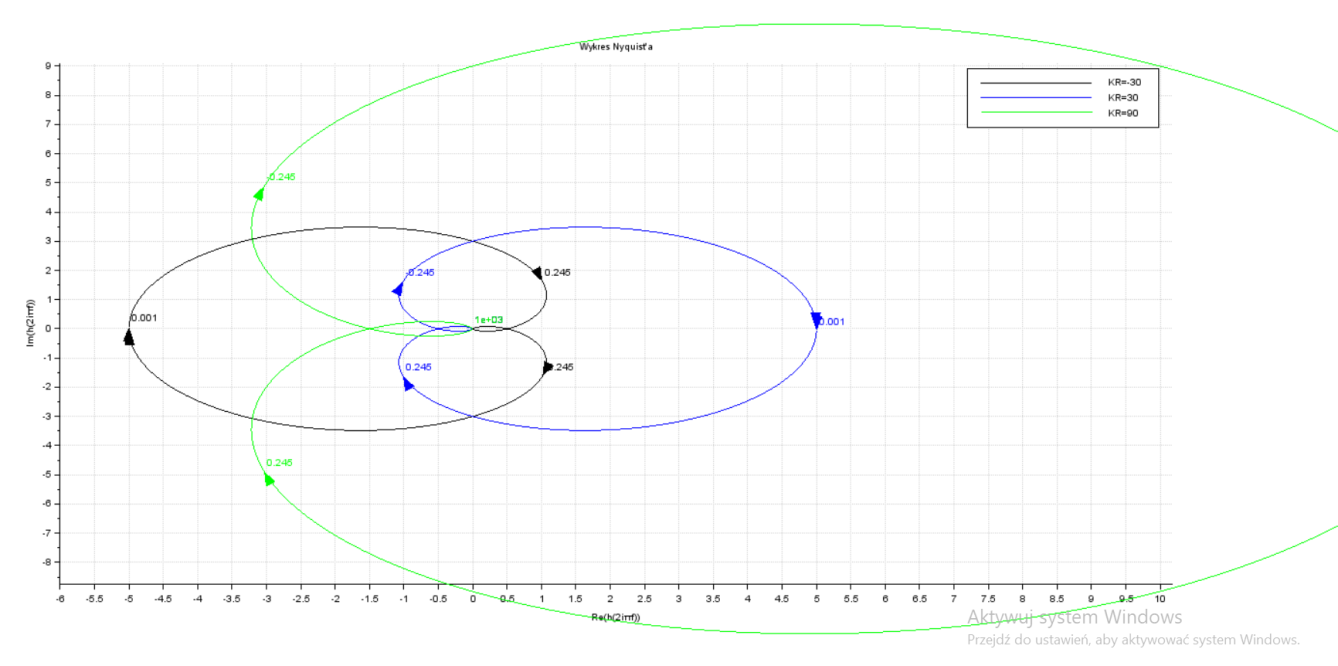
\includegraphics[width=12cm]{nq1.png}
            \centering
        \end{figure}

        \begin{figure}[h!]
            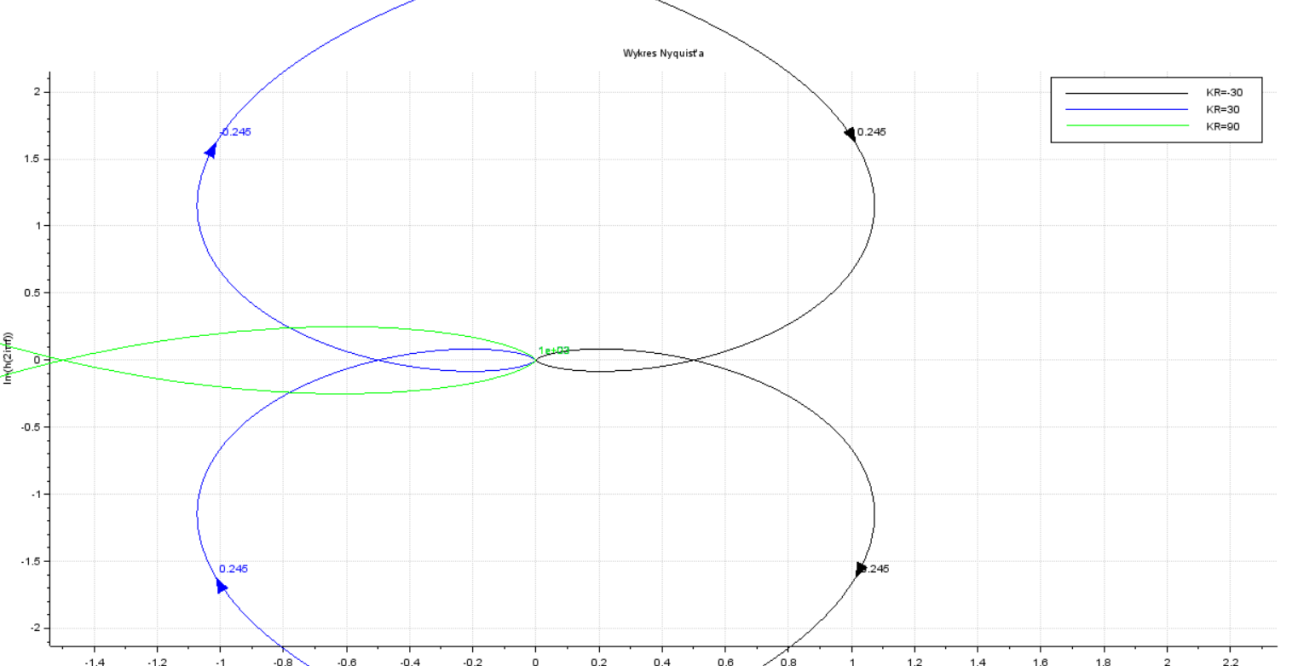
\includegraphics[width=12cm]{nq2.png}
            \centering
        \end{figure}
        Więc syste zamknięty jest stabilny.
        \\ \textbf{Uchyb}\\
        $Y_0(t)=1$
        $$K_E=\frac{\left(s + 1\right) \left(s + 2\right) \left(s + 3\right)}{k + \left(s + 1\right) \left(s + 2\right) \left(s + 3\right)}$$
        $$\varepsilon=\lim_{s \rightarrow 0} {s\cdot K_E\cdot Y_0}=\frac{6}{k + 6}$$
        
        \newpage 
        
        \item $K_{OLS}=\frac{k}{\left(s + 1\right)^{2} \left(s + 2\right)}$
        
        
        Wykres Nyquista dla OLS:
        $$K_{OLS}=\frac{k}{\left(s + 1\right)^{2} \left(s + 2\right)}$$
        
        \begin{figure}
            \centering
            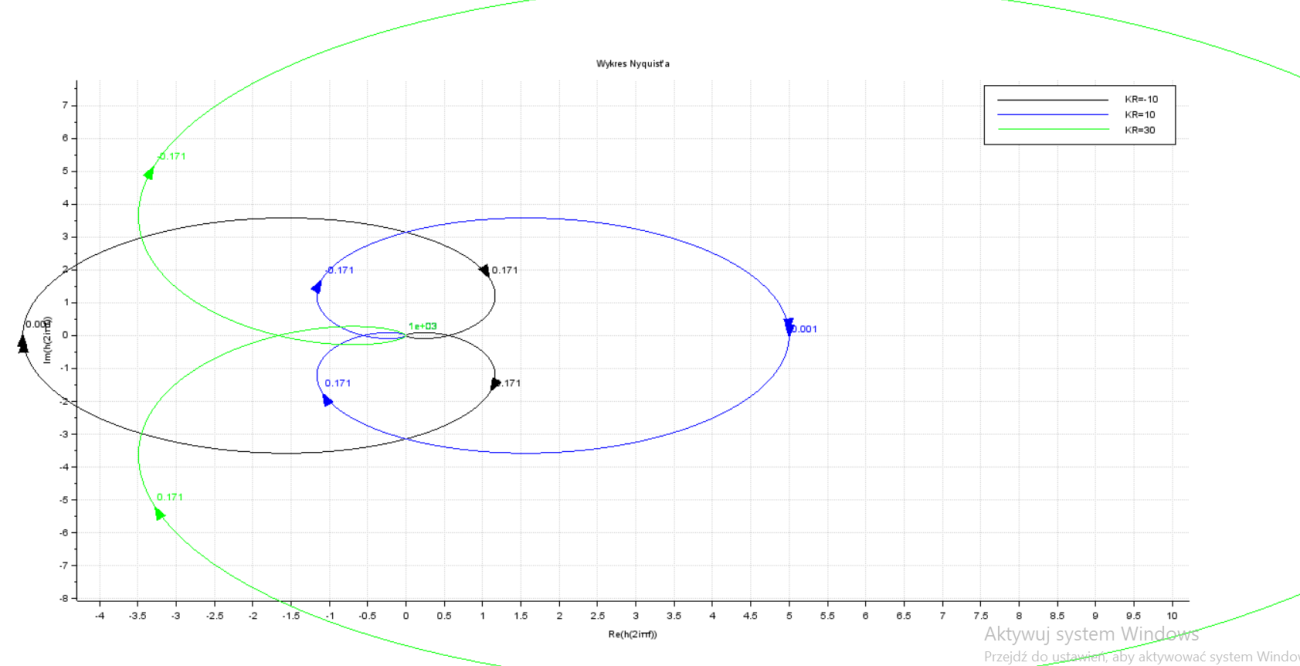
\includegraphics[width=12cm]{nq3.png}\
        \end{figure}
        
        System zamknięty jest stabilny.\\
        \\ \textbf{Uchyb}\\
        Dla $Y_0(t)=1$
        $$K_E=\frac{\left(s + 1\right)^{2} \left(s + 2\right)}{k + \left(s + 1\right)^{2} \left(s + 2\right)}$$
        $$\varepsilon=\lim_{s \rightarrow 0} {s\cdot K_E\cdot Y_0}=\frac{2}{k + 2}$$
        %oceniam stabilnosc recznie
    \end{enumerate}
\end{enumerate}
    \newpage
    
        
        
    \section*{Zadanie 3}
    \begin{enumerate}[a)]
        \item $K_O=\frac{1}{s \left(s + 1\right) \left(s + 2\right)}$ 
        
        $$K_R=k$$
        $$G=1$$
        Transmitancja systemu zamknietego:
        $$K_Z=\frac{K_O\cdot K_R}{1+K_O\cdot K_RG}=\frac{k}{k + s \left(s + 1\right) \left(s + 2\right)}$$
        Transmitancja systemu otwartego:
        $$K_O=K_O\cdot K_R\cdot G=\frac{k}{s \left(s + 1\right) \left(s + 2\right)}$$
        Sprawdzamy stabilność CLS z pomocą kryterium Hurwitza:\\
        Wielomian charakterystyczny CLS:
        $$M_Z=k + s \left(s + 1\right) \left(s + 2\right)$$
        %macierze
        Macierz Hurwitza:
        
    $$H_{3}=\left[\begin{matrix}3 & k & 0\\1 & 2 & 0\\0 & 3 & k\end{matrix}\right]$$
        
        Wyznacznik:$$W=- k^{2} + 6 k$$ Wyznacznik dodatni gdy: $0 < k \wedge k < 6$\newline
        Wyznacznik:$$W=6 - k$$ Wyznacznik dodatni gdy: $k < 6$\newline
        Wyznacznik:$$W=3$$ Wyznacznik dodatni zawsze\newline
        CLS stabilny gdy $k\in (0,6)$\newpage 
        \textbf{Uchyby}
        %nyquist
        $$K_E=\frac{\left(s + 1\right) \left(s + 2\right) \left(s + 3\right)}{k + \left(s + 1\right)
        \left(s + 2\right) \left(s + 3\right)}$$
        Dla $Y_0(t)=1$
        $$\varepsilon=\lim_{s \rightarrow 0} {s\cdot K_E\cdot Y_0}=0$$\\
        Dla $Y_0(t)=t$
        $$\varepsilon=\lim_{s \rightarrow 0} {s\cdot K_E\cdot Y_0}=\frac{2}{k}$$\\
        Dla $Y_0(t)=t^2$
        $$\varepsilon=\lim_{s \rightarrow 0} {s\cdot K_E\cdot Y_0}=\infty \operatorname{sign}{\left(\frac{1}{k} \right)}$$\\
        Dla $Y_0(t)=1+t$
        $$\varepsilon=\lim_{s \rightarrow 0} {s\cdot K_E\cdot Y_0}=\frac{2}{k}$$\\
        \item $K_O=\frac{1}{\left(s + 1\right) \left(s + 2\right)}$
        
        
        $$K_R=\frac{k}{s}$$
        $$G=1$$
        Transmitancja CLS:
        $$K_Z=\frac{K_O\cdot K_R}{1+K_O\cdot K_RG}=\frac{\frac{1}{\left(s + 1\right) \left(s + 2\right)}\cdot \frac{k}{s}}{1+\frac{1}{\left(s + 1\right) \left(s + 2\right)}\cdot \frac{k}{s}\cdot 1}=\frac{k}{k + s \left(s + 1\right) \left(s + 2\right)}$$
        Transmitancja OLS:
        $$K_O=K_O\cdot K_R\cdot G=\frac{k}{s \left(s + 1\right) \left(s + 2\right)}$$

        Uchyby dalej są takie same jak w poprzednim przykładzie.
    \end{enumerate}
        
        \section*{Zadanie 4}
    
$$K_O=\frac{1}{\left(s - 3\right) \left(s + 1\right) \left(s + 2\right)}$$
$$K_R=k$$
$$G=1$$
Transmitancja CLS:
$$K_Z=\frac{K_O\cdot K_R}{1+K_O\cdot K_RG}=\frac{\frac{1}{\left(s - 3\right) \left(s + 1\right) \left(s + 2\right)}\cdot k}{1+\frac{1}{\left(s - 3\right) \left(s + 1\right) \left(s + 2\right)}\cdot k\cdot 1}=\frac{k}{k + s^{3} - 7 s - 6}$$
Transmitancja OLS:
$$K_O=K_O\cdot K_R\cdot G=\frac{k}{\left(s - 3\right) \left(s + 1\right) \left(s + 2\right)}$$
\textbf{Sprawdzamy stabilność CLS z pomocą kryterium Hurwitza:}\newline
Wielomian charakterystyczny CLS:
$$M_Z=k + s^{3} - 7 s - 6$$
 %macierze
Macierz Hurwitza na podstawie tego wielomianu oraz wartości wyznacznika i podwyznaczników:

$$H_{3}=\left[\begin{matrix}0 & k - 6 & 0\\1 & -7 & 0\\0 & 0 & k - 6\end{matrix}\right]$$

Wyznacznik:$$W=- \left(k - 6\right)^{2}$$ Wyznacznik dodatni gdy: $\text{False}$\newline
Wyznacznik:$$W=6 - k$$ Wyznacznik dodatni gdy: $-\infty < k \wedge k < 6$\newline
Wyznacznik:$$W=0$$ Wyznacznik dodatni gdy: False\newline
CLS jest zawsze nie stabilny\
\textbf{Uchyb}\
$$K_E=\frac{s^{3} - 7 s - 6}{k + s^{3} - 7 s - 6}$$
 Dla $Y0(t)=1$
$$\varepsilon=\lim{s \rightarrow 0} {s\cdot K_E\cdot Y_0}=- \infty \operatorname{sign}{\left(\frac{1}{k - 6} \right)}$$
        
        \end{document}
        